% !TEX program = xelatex
\documentclass[10pt,a4paper]{article}

% ======================== 基础包 ========================
\usepackage[top=0.55cm,bottom=0.5cm,left=1.0cm,right=1.0cm]{geometry}
\usepackage{ctex}
\usepackage{titlesec}
\usepackage{enumitem}
\usepackage{xcolor}
\usepackage{graphicx}
\usepackage{hyperref}
\usepackage{fontawesome5}
\usepackage{tikz}

% ======================== 颜色定义 ========================
\definecolor{primary}{HTML}{2B4C7E}
\definecolor{darktext}{HTML}{2D2D2D}
\definecolor{graytext}{HTML}{666666}
\definecolor{rulecolor}{HTML}{B0B0B0}
\definecolor{photoframe}{HTML}{8C99AD}

% ======================== 超链接 ========================
\hypersetup{
    colorlinks=true, linkcolor=primary, urlcolor=primary,
    pdfauthor={徐其栋}, pdftitle={徐其栋 - 求职简历}
}

% ======================== 字体设置 ========================
\setCJKmainfont{SimHei}[BoldFont=SimHei]
\setmainfont{Segoe UI}[BoldFont=Segoe UI Bold]

% ======================== 段落和间距 ========================
\setlength{\parindent}{0pt}
\setlength{\parskip}{0pt}
\pagestyle{empty}

% ======================== 标题样式 ========================
\titleformat{\section}
    {\large\bfseries\color{primary}}
    {}{0em}{}
    [\vspace{-0.5em}{\color{rulecolor}\rule{\textwidth}{0.6pt}}\vspace{-0.2em}]
\titlespacing*{\section}{0pt}{0.55em}{0.3em}

% ======================== 自定义命令 ========================
\newcommand{\projectblock}[3]{%
    {\bfseries\color{darktext}#1}\hfill{\color{graytext}#2}\\%
    {\small\color{graytext}#3}%
    \vspace{0.15em}%
}

% ======================== 文档开始 ========================
\begin{document}

% ======================== 头部：左信息 + 右照片 ========================
\begin{minipage}[b]{0.72\textwidth}
    {\fontsize{25}{30}\selectfont\bfseries\color{primary}徐其栋}\\[10pt]
    {\small\color{primary}%
    \faBirthdayCake\hspace{0.35em}23 岁\hspace{0.75em}{\color{rulecolor}·}\hspace{0.75em}%
    \faUserGraduate\hspace{0.35em}2026 届应届生\hspace{0.75em}{\color{rulecolor}·}\hspace{0.75em}%
    \faYenSign\hspace{0.35em}期望薪资 5K--8K}\\[7pt]
    {\small\color{graytext}%
    \faPhone\hspace{0.35em}17268891140\hspace{0.75em}{\color{rulecolor}/}\hspace{0.75em}%
    \faEnvelope\hspace{0.35em}\href{mailto:xqd922@outlook.com}{xqd922@outlook.com}\hspace{0.75em}{\color{rulecolor}/}\hspace{0.75em}%
    \faGlobe\hspace{0.35em}\href{https://1001.pp.ua}{1001.pp.ua}}
\end{minipage}\hfill
\begin{minipage}[b]{0.25\textwidth}
    \raggedleft
    {\setlength{\fboxsep}{0pt}\setlength{\fboxrule}{0.7pt}%
     \color{photoframe}\fbox{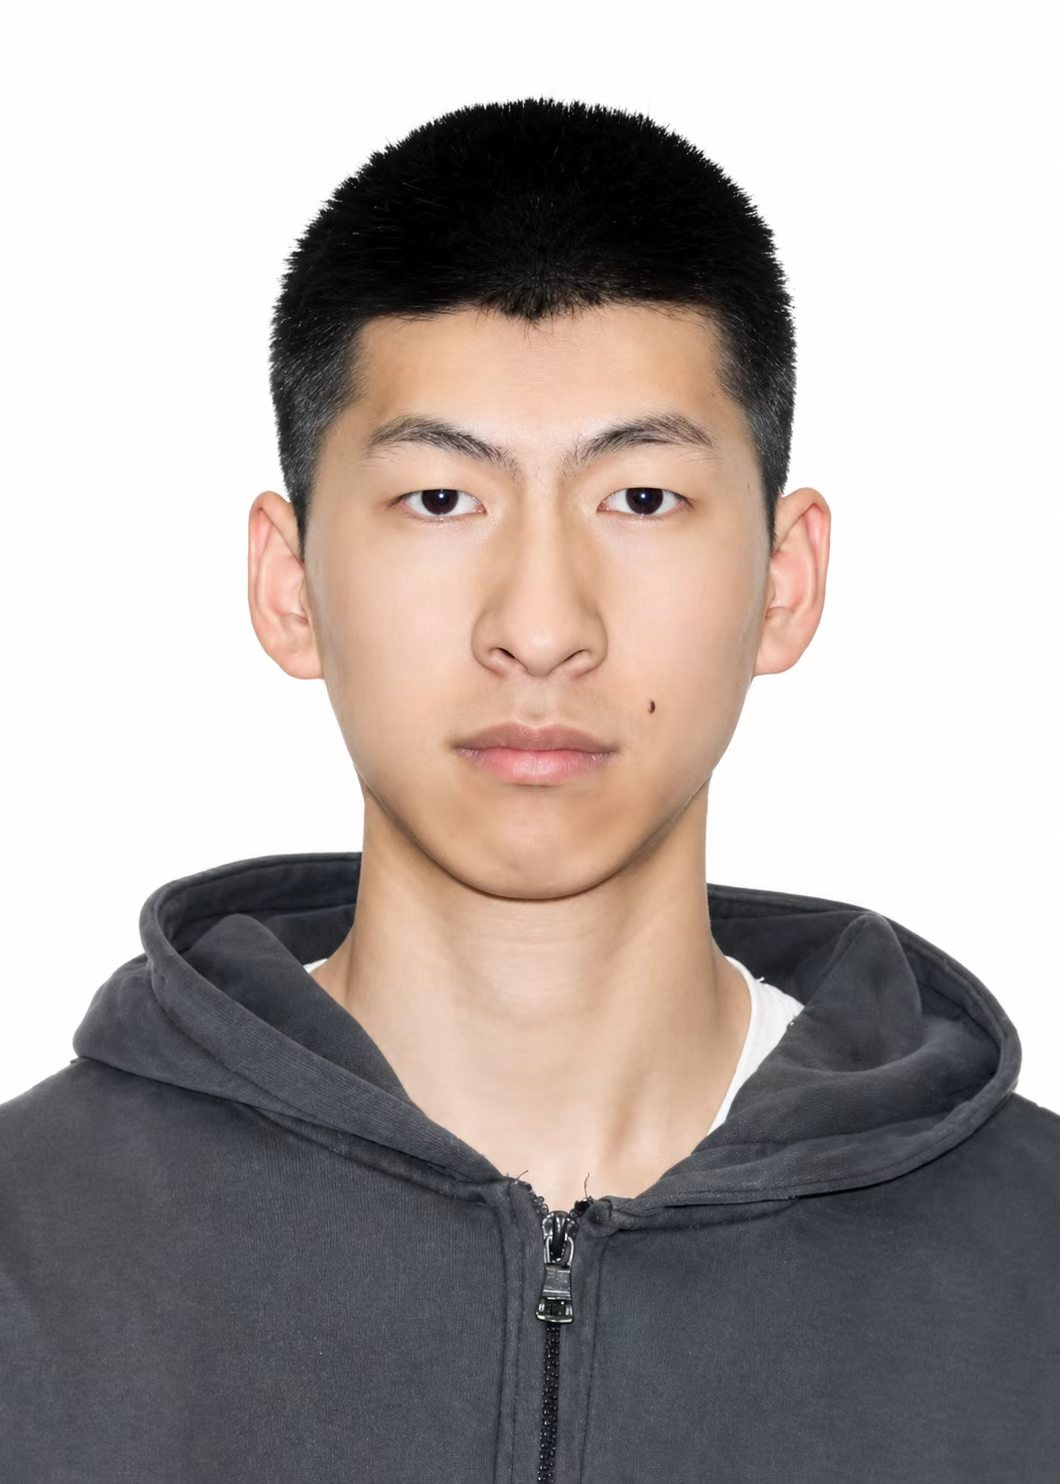
\includegraphics[height=3.0cm]{photo.jpg}}}
\end{minipage}

\vspace{2pt}
{\color{primary}\rule{\textwidth}{1.1pt}}

% ======================== 教育背景 ========================
\section{\faGraduationCap\hspace{0.4em}教育背景}

{\bfseries 滇西科技师范学院}\hspace{0.7em}{\color{graytext}2022.09 -- 2026.07}\hfill{\bfseries 物联网工程\hspace{0.3em}|\hspace{0.3em}本科}

\vspace{0.2em}

{\color{darktext}\textbf{主修课程：}C 语言、单片机原理、嵌入式技术、计算机网络、传感器原理、数字电子技术、模拟电子技术}

% ======================== 专业技能 ========================
\section{\faCogs\hspace{0.4em}专业技能}

{\bfseries\color{primary}嵌入式 / 物联网：}\hspace{0.3em}{\color{darktext}STM32、外设驱动调试、I2C、UART、PWM、MQTT、蓝牙、Wi-Fi、FreeRTOS}

\vspace{2pt}

{\bfseries\color{primary}编程与数据库：}\hspace{0.3em}{\color{darktext}C 语言、C++、Python、Qt、MySQL}

\vspace{2pt}

{\bfseries\color{primary}开发工具：}\hspace{0.3em}{\color{darktext}Keil MDK、Visual Studio、Git、Linux、嘉立创 EDA、示波器 / 逻辑分析仪}

% ======================== 实习经历 ========================
\section{\faBriefcase\hspace{0.4em}实习经历}

{\bfseries 云南航天工程物探检测股份有限公司}\hfill{\color{graytext}嵌入式软件开发实习生\hspace{0.3em}·\hspace{0.3em}2025.08 -- 2025.12}

{\small\color{graytext}业务场景：隧道 / 桥梁 / 路面工程检测设备\hspace{0.3em}|\hspace{0.3em}MCU 嵌入式软件\hspace{0.3em}|\hspace{0.3em}C/C++\hspace{0.3em}|\hspace{0.3em}外设驱动\hspace{0.3em}|\hspace{0.3em}传感器采集\hspace{0.3em}|\hspace{0.3em}软硬件联调\hspace{0.3em}|\hspace{0.3em}Git}

\vspace{2pt}

\begin{itemize}[leftmargin=1.5em, itemsep=1pt, parsep=0pt, topsep=2pt]
    \item \textbf{采集节点固件开发}：基于 MCU 平台使用 C/C++ 开发检测设备采集节点固件，完成传感器外设驱动与数据的采集、滤波、处理，将原始信号整理为上层可用的检测数据。
    \item \textbf{检测数据显示与人机交互}：实现检测数据的实时显示与设备操作界面，按现场作业流程重排交互逻辑，减少单次检测的重复操作。
    \item \textbf{联调与问题定位}：参与设备软硬件联调，定位并修复程序缺陷与通信异常，形成从信号、通信到程序的分层排查思路；使用 Git 进行分支管理与版本迭代。
\end{itemize}

\vspace{0.2em}

% ======================== 项目经历 ========================
\section{\faProjectDiagram\hspace{0.4em}项目经历}

\projectblock{四足物联网机器狗控制系统}{2025.03 -- 2025.04}{技术栈：STM32F407ZE\hspace{0.3em}|\hspace{0.3em}PCA9685\hspace{0.3em}|\hspace{0.3em}MPU6050\hspace{0.3em}|\hspace{0.3em}ESP32\hspace{0.3em}|\hspace{0.3em}WS2812\hspace{0.3em}|\hspace{0.3em}I2C / UART\hspace{0.3em}|\hspace{0.3em}二维逆运动学}

\begin{itemize}[leftmargin=1.5em, itemsep=1pt, parsep=0pt, topsep=2pt]
    \item \textbf{多舵机运动控制}：构建 STM32F407ZE $\rightarrow$ I2C $\rightarrow$ PCA9685 $\rightarrow$ 8 路舵机控制链路，利用 16 路 12 位 PWM 扩展驱动四腿 8 个关节，实现站立、前进、后退、转向等共 9 种动作与姿态。
    \item \textbf{逆运动学与平滑控制}：基于二维二连杆模型，由足端目标坐标 $(x, y)$ 反解大小腿关节角；增加目标点几何可达性校验及 0\textdegree--180\textdegree{} 关节限幅，并以 1\textdegree{} 步进插值分解目标角度，降低指令阶跃造成的机械冲击与抖动。
    \item \textbf{姿态检测与多模交互}：通过 I2C 读取 MPU6050 三轴加速度与三轴角速度数据，完成倾倒判断和状态反馈；经 USART2 接入蓝牙控制链路并由网页端下发动作指令，ESP32 通过 UART4 接入语音控制指令，WS2812 显示系统运行状态。
\end{itemize}

\vspace{0.15em}

\projectblock{STM32 智能交互台灯控制系统}{2026.03 -- 2026.05}{技术栈：STM32F103C8T6\hspace{0.3em}|\hspace{0.3em}PCB 设计\hspace{0.3em}|\hspace{0.3em}ADC / TIM2 PWM\hspace{0.3em}|\hspace{0.3em}HC-SR04\hspace{0.3em}|\hspace{0.3em}红外感应\hspace{0.3em}|\hspace{0.3em}USART2/3\hspace{0.3em}|\hspace{0.3em}OLED}

\begin{itemize}[leftmargin=1.5em, itemsep=1pt, parsep=0pt, topsep=2pt]
    \item \textbf{控制板设计与驱动联调}：基于 STM32F103C8T6 独立完成控制板 PCB 设计，完成 OLED、ADC 光敏、红外、HC-SR04、蓝牙及语音模块的外设驱动与软硬件联调。
    \item \textbf{四模式控制与 PWM 调光}：实现自动、手动、蓝牙、语音 4 种控制模式；自动模式采集环境光 ADC 数据，通过 TIM2 PWM 完成多档亮度调节，并根据不同输入切换对应控制逻辑。
    \item \textbf{传感器融合与人机交互}：结合红外在位检测和 HC-SR04 距离数据，实现无人自动关灯与近距离报警；OLED 显示亮度档位及模式，USART2/3 分别接收蓝牙和语音控制指令，完成“感知--决策--执行--显示”完整链路。
\end{itemize}

\vspace{0.15em}

% ======================== 个人评价 ========================
\section{\faUser\hspace{0.4em}个人评价}

性格踏实、积极主动，有较强的 \textbf{上进心与自驱力}，抗压能力好、\textbf{可接受加班、服从安排}；对嵌入式开发有浓厚兴趣，能快速融入团队，希望在该方向长期深耕、与公司共同成长。

\end{document}
